% Editable report section: Implementation and the AI-Assisted Coding Process
\section{Implementation and the AI-Assisted Coding Process}
\label{sec:4}

The site handler first locates the live arc above the new site. For an ordinary split it keeps the left arc identity, inserts the new site's arc and a right copy of the original site's arc, records their separating edge, then reschedules affected neighbours. Equal-height sites use an adjacent limiting arc instead of dividing by a zero directrix gap.

\begin{lstlisting}[caption={Local arc insertion during a site event.},label={lst:1}]
new, right = Arc(site), Arc(old.site)
self.beach.insert_after(old, new)
self.beach.insert_after(new, right)
self.edge(old.site, site)
for arc in (before, old, new, right, after):
    self.schedule(arc)
\end{lstlisting}

The circle handler verifies identity and generation before changing topology. It records the vertex on the two disappearing boundaries and on the newly created boundary, removes the middle arc and reschedules the surviving pair. These operations are local even though the output affects three cells.

\begin{lstlisting}[caption={Boundary updates during a valid circle event.},label={lst:2}]
self.edge(left.site, middle.site, vertex)
self.edge(middle.site, right.site, vertex)
self.edge(left.site, right.site, vertex)
self.beach.remove(middle)
self.statistics["circle_events"] += 1
self.schedule(left)
self.schedule(right)
\end{lstlisting}

AI-generated code was integrated incrementally: geometry passed ten tests, geometry plus AVL operations seventeen, and queue/circle examples twenty-one. The first complete cell suite then produced three genuine failures. Independent checks prompted corrections to clipping and numerical construction, documented in Section~\ref{sec:6}.

The snippets above are excerpts from the actual source. Complete editable modules and a companion source listing are included in the package. No public implementation was copied into the algorithmic core.

\subsection{Interfaces, Exports and Native Display}

The file parser accepts one whitespace- or comma-separated pair per line, ignores blank lines and comments, and reports malformed line numbers. Seeded generation uses Python's random generator. Exact duplicates retain their input-index groups. Batch commands print counts and construction timing, then optionally write an image, CSV and JSON.

\begin{figure}[!htbp]
\centering
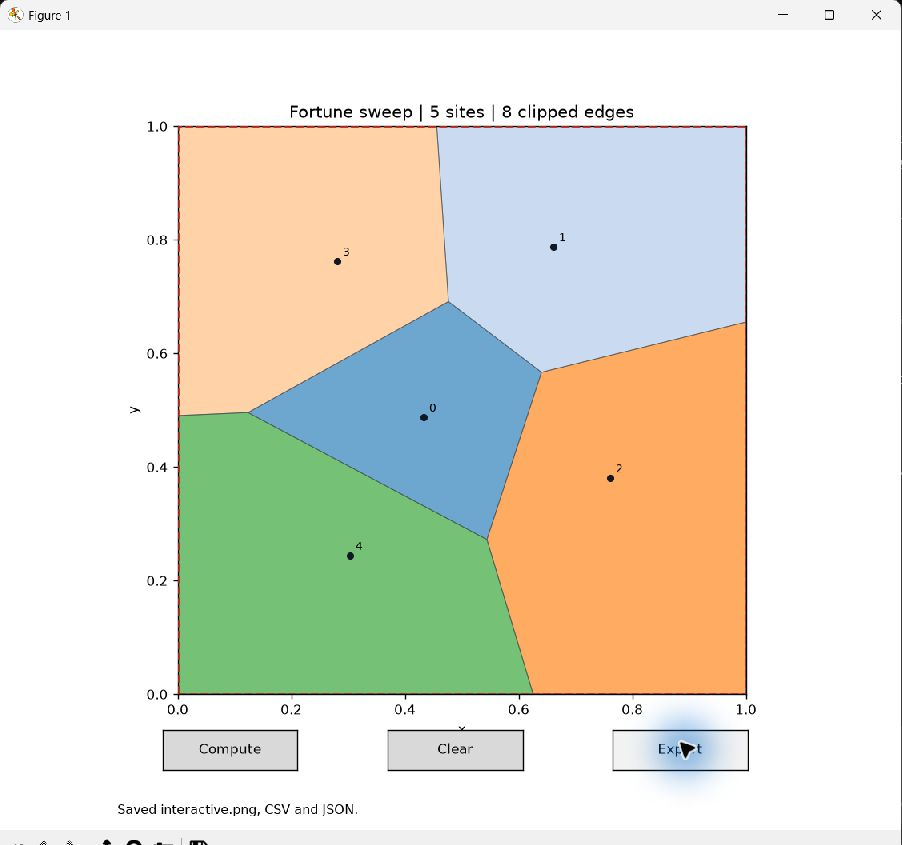
\includegraphics[width=0.92\linewidth,height=0.55\textheight,keepaspectratio]{gui-native.png}
\caption{Native Windows interface after a successful five-site export.}
\label{fig:4}
\end{figure}

The interface supports click insertion, Compute, Clear, Export and Animate. Callback tests exercise input and output; native Export produced PNG, CSV and JSON. Figure~\ref{fig:4} is a real capture of the earlier interface, before Animate was added. Its five-site state is retained in \path{examples/interactive.json}.

CSV rows give ordered vertices, next endpoints, neighbours and ray information. JSON includes defining sites and ray origins/directions. Static rendering supports an off-screen backend; interactive rendering needs a GUI backend \cite{matplotlibbackends}.

\subsection{Pointer-Controlled Sweep Replay}

Animate, or \code{--animate}, exports offline HTML. Python records live arc orders, queue previews, stale flags and edges from \code{FortuneSweep.step()}. Pointer movement selects a state by binary search; Canvas draws its parabolas as quadratic Bezier curves without rerunning Fortune. Play and Next event expose the same sequence. Appendix~\ref{sec:c} provides the capture and measurements.

The educational history can occupy $O(n^2)$ space and is capped at 200 distinct sites. It is excluded from ordinary $O(n\log n)$ construction benchmarks. The viewer explicitly identifies the production sorted-neighbour special case for collinear/minimal inputs.
